\documentclass{article}

% if you need to pass options to natbib, use, e.g.:
%     \PassOptionsToPackage{numbers, compress}{natbib}
% before loading neurips_2020

% ready for submission
% \usepackage{neurips_2020}

% to compile a preprint version, e.g., for submission to arXiv, add add the
% [preprint] option:
%     \usepackage[preprint]{neurips_2020}

% to compile a camera-ready version, add the [final] option, e.g.:
%	\usepackage[final]{neurips_2020}

% to avoid loading the natbib package, add option nonatbib:
%	\usepackage[nonatbib]{neurips_2020}
\usepackage[final]{neurips_2020}

\usepackage[utf8]{inputenc} % allow utf-8 input
\usepackage[T1]{fontenc}    % use 8-bit T1 fonts
\usepackage{hyperref}       % hyperlinks
\usepackage{url}            % simple URL typesetting
\usepackage{booktabs}       % professional-quality tables
\usepackage{amsfonts}       % blackboard math symbols
\usepackage{amsmath}
\usepackage{nicefrac}       % compact symbols for 1/2, etc.
\usepackage{microtype}      % microtypography
\usepackage{multicol}
\usepackage{graphicx}

\title{Structural Compression of ResNet-like Convolutional Neural Networks}

% The \author macro works with any number of authors. There are two commands
% used to separate the names and addresses of multiple authors: \And and \AND.
%
% Using \And between authors leaves it to LaTeX to determine where to break the
% lines. Using \AND forces a line break at that point. So, if LaTeX puts 3 of 4
% authors names on the first line, and the last on the second line, try using
% \AND instead of \And before the third author name.

\author{%
	Nicholas~Kastanos (nk569), Queens' College \\
	Department of Computer Science and Technology\\
	University of Cambridge\\
	Cambridge, CB3 0FD\\
	\texttt{nk569@cam.ac.uk} \\
}

\begin{document}
	
	\maketitle
	
	\begin{abstract}
		abstract
	\end{abstract}
	
	\section{Introduction}
	
	
	
	% objectives and purpose
	
	\section{Related Work}
	%reasons behind work	
	% can discuss relationships between existing knowledge and what is being done here	
	\subsection{ResNet}
	
	The residual block first postulated for use in ResNet has become a common-place feature in many subsequent networks (DenseNet, Inception). 
	% ResNet https://arxiv.org/abs/1512.03385
	% ResNet50V2 https://arxiv.org/abs/1603.05027
	
	\subsection{Separable convolutions}
	
	Convolution Layers contain a vast majority of the parameters in modern CNNs. By targeting parameter reductions to these layers, the compression can be spread throughout the network. Separable convolutions reduce the number of parameters by separating the convolution into multiple stages through spatially and depthwise separable convolutions. While these convolutions reduces the memory and computation requirements of the system, the reduction in parameters reduces the number of possible kernels explored in training, and the resulting network may be suboptimal.
	
	\subsubsection{Spatially separable convolutions}
	
	% References: Spatially Separable
	% Inception v4: https://arxiv.org/pdf/1512.00567v3.pdf
	% SqueezeNet mentions it https://arxiv.org/pdf/1602.07360.pdf
	% MobileNet: https://arxiv.org/abs/1704.04861
	
	A convolution kernel can be decomposed on its 2D spatial axis, i.e. height and width. Conceptually, the $n \times n$ kernel can be separated into two smaller kernels, a $n \times 1$ followed by a $1 \times n$ kernel. These kernels can be applied in sequential convolutions to obtain the same output shape as the single convolution. These decomposed kernels scale the parameters required by the convolution by a factor $P_s(n)$ (see Equation~\ref{eqn:spat_params}). 
	
	Similarly, the multiplication operations of a spatially separated convolution are reduced. For a $M \times M$ input convolved with a $n \times n$ kernel, the number of multipications are reduced by a factor of $M_s(n)$ (see Equation~\ref{eqn:spat_ops}). 
	
	Equations~\ref{eqn:spat_params})~and~\ref{eqn:spat_ops} show that spatially separable convolutions show computational benefits when $n > 2$. 
	
	\begin{multicols}{2}
		\begin{equation}\label{eqn:spat_params}
			P_s(n) = \frac{2}{n}
		\end{equation}
	\break
		\begin{equation}\label{eqn:spat_ops}
			\begin{split}
				M_s(M, n) = & \frac{2}{n} + \frac{2}{n(M-2)} \\
				\Rightarrow M_s(n) = & \frac{2}{n},~\text{where}~M >> n
			\end{split}
		\end{equation}		
	\end{multicols}
	
	\subsubsection{Depthwise separable convolutions}	
	% Depthwise Separable
	% MobileNet https://arxiv.org/abs/1704.04861
	% Xception: https://arxiv.org/abs/1610.02357
	
	Depthwise separable convolutions separate the spatial convolution from the depth of the filters. This is accomplished by an initial depthwise convolution, followed by a pointwise convolution. The initial depthwise convolution separates the channels of the input and kernel, and convolves them independently. The pointwise convolution is a $N_F \times 1 \times 1 \times N_C$ convolution where $N_F$ and $N_C$ are the number of filters and channels respectively. 
	
	The number of parameters $P_d(n)$ and multiplications $M_d(n)$ are reduced by the same factor, which can be seen in Equation~\ref{eqn:depthwise}. Many CNNs have $N_F >> 1$, therefore depthwise convolutions show compression kernel sizes greater than 1. 

	\begin{equation} \label{eqn:depthwise}
		P_d(n) = M_d(n) = \frac{1}{n^2} + \frac{1}{N_F} \approx \frac{1}{n^2}
	\end{equation}
	
%	\subsection{Quantised Training} I dont know if I want to do this anymore. Maybe just post trainng quantization
	
	\subsection{Quantization and datatype compression}
	
	%	https://ieeexplore.ieee.org/abstract/document/8524017
	Many resource-constrained devices do not have sufficient memory to use large neural networks, or may not have access to floating-point arithmetic units. Both of these factors can be mitigated by using low-precision integer datatypes, such as 8-bit integers. This effectively reduces the memory required for each parameter by \nicefrac{1}{4}. 
	
	However, by reducing the precision of the datatype, the learned parameters are not represeted fully, reducing the performance of the network. This has been shown to have significant effect on the network when reducing 32-bit floating point numbers to 8-bit integers, however quantization aware training can limit the impact. 
	%	https://papers.nips.cc/paper/2018/file/e82c4b19b8151ddc25d4d93baf7b908f-Paper.pdf
	
	TensorFlow, by default, uses 32-bit floating point precision for its network layers and training. TensorFlow Lite provides functionality to convert trained models to quantized, 8-bit integer models, however it does not have native 8-bit implementations for all layer types. In the event an incompatible layer is used, the engine upscales the activations to the full precision for that layer.
	
	\section{Methodology}
	% Use ResNet50V2
	In order to asses the benefits and costs of the compression, a baseline architecture is established and used as a comparison reference point. The ResNet50V2 image classification CNN-based neural network is used as the baseline architecture. The baseline architecture and subsequent networks are trained using the same parameters using TensorFlow. 
	
	\subsection{Training}
	%% how were the networks trained
	
	% Use of datasets CIFAR10
	The CNNs are trained using the CIFAR-10 dataset, with random horizontal flips, rotations, and cropping. The Adam optimizer is used with a learning rate of $0.001$, and categorical crossentropy loss. The networks are trained for 30 epochs with a batch size of 32. 
	
	\subsection{Modified residual blocks}
	
	\begin{figure}[h!]
		\centering
		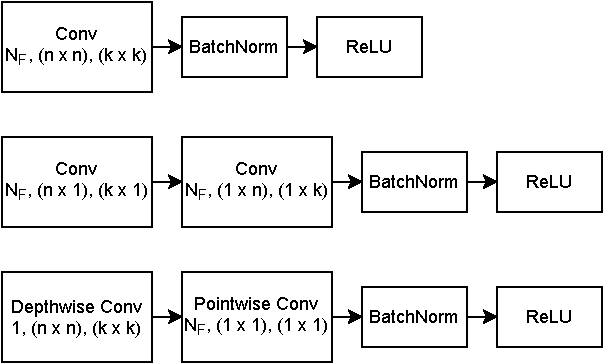
\includegraphics[width=0.5\textwidth]{images/conv-structure.pdf}
		\caption{Example of replaced convolutions with separable convolutions with $N_F$ filters, kernel size $n$, and stride $k$. From top to bottom: Traditional Convolution; Spatially Separable Convolution; Depthwise Separable Convolution}
		\label{fig:conv-structure}
	\end{figure}
	
		% How were convolutions separated / chosen for separation
	In order to modify the ResNetV2 network, the convolutions in the residual blocks are chosen to be substituted with separable convolutions. Additional batch normalization and activation layers are not added between these new layers. An example of this expansion can be seen in Figure~\ref{fig:conv-structure}. Only convolutions which would provide parameter and compute reduction are replaced with separable convolutions. For ResNet50V2, these are any convolutions where the kernel size $n > 1$.
	
	These two additional CNNs are called ResNet50V2-Spatial and ResNet50V2-Depthwise, where convolutional layers are replaced with spatial and depthwise convolutions respectively. 
	
	% \subsection{Quantization-aware Training}
	
	\subsection{Post-training quantization}
	% How were layers quantized
	The fully trained models are compressed to 8-bit precision using TensorFlow Lite. The framework recommends the provision of the representative dataset to enhance the optimization process. This allows for quantization of both weights and activations for quantizable operations. The representative dataset is compiled using 1000 samples from the dataset. 	
	
	
	\section{Evaluation and results}
	
	\begin{table}
		\caption{Results}
		\label{tbl:results}
		\centering
		\begin{tabular}{llll}
			\toprule
			Name                            & Loss & Accuracy (\%) & Size (MB) \\ \midrule
			ResNet50V2                      & 0    & 100           & 20000     \\
			ResNet50V2-Spatial              & 0    & 100           & 2000      \\
			ResNet50V2-Depthwise            & 0    & 100           & 2000      \\
			Compressed ResNet50V2           & 0    & 100           & 20000     \\
			Compressed ResNet50V2-Spatial   & 0    & 100           & 2000      \\
			Compressed ResNet50V2-Depthwise & 0    & 100           & 2000      \\ \bottomrule
		\end{tabular}
	\end{table}
	
	% include implications of results
	%Limitations
	
	\section{Conclusion}
	
	
	
%	\begin{table}
%		\caption{Sample table title}
%		\label{sample-table}
%		\centering
%		\begin{tabular}{lll}
%			\toprule
%			\multicolumn{2}{c}{Part}                   \\
%			\cmidrule(r){1-2}
%			Name     & Description     & Size ($\mu$m) \\
%			\midrule
%			Dendrite & Input terminal  & $\sim$100     \\
%			Axon     & Output terminal & $\sim$10      \\
%			Soma     & Cell body       & up to $10^6$  \\
%			\bottomrule
%		\end{tabular}
%	\end{table}
%	

	
\end{document}